\documentclass[conference]{IEEEtran}
\IEEEoverridecommandlockouts
% The preceding line is only needed to identify funding in the first footnote. If that is unneeded, please comment it out.
\usepackage[utf8]{inputenc}
\usepackage[greek,english]{babel}
\usepackage{alphabeta}
\usepackage{cite}
\usepackage{amsmath,amssymb,amsfonts}
\usepackage{algorithmic}
\usepackage{graphicx}
\usepackage{textcomp}
\usepackage{xcolor}
\usepackage{pgfplots}
\usepackage{xcolor}
\usepackage{listings}
\usepackage{hyperref} 
\usepackage{pgfplots}

\lstset{basicstyle=\ttfamily,
  showstringspaces=false,
  commentstyle=\color{red},
  keywordstyle=\color{blue}
}
\pgfplotsset{compat=1.16}

\def\BibTeX{{\rm B\kern-.05em{\sc i\kern-.025em b}\kern-.08em
    T\kern-.1667em\lower.7ex\hbox{E}\kern-.125emX}}
\begin{document}

\title{Key-Value stores Riak vs ArangoDB \\

}

\author{\IEEEauthorblockN{Αγγελου Στελιος}
\IEEEauthorblockA{
% \textit{National Technical University of Athens} \\
% \textit{Electrical and Computer Egineering}\\
αριθμος μητρώου
}
\and
\IEEEauthorblockN{Γκέργκες Μάρκος}
\IEEEauthorblockA{
03117870 
}
\and
\IEEEauthorblockN{Παπαβασιλόπουλος Παναγιώτης-Φίλιππος}
\IEEEauthorblockA{
03117444
}
}

\maketitle

\begin{abstract}
    Τα τελευταία χρόνια η ανάπτυξη των συστημάτων 
διαχείρισης βάσεων δεδομένων (DBMS) είναι αναπόφευκτη προκειμένου να 
ανταποκριθούμε στη ραγδαία αύξηση των δεδομένων που 
αποθηκεύονται. Στην προσπάθεια διαχείρισης big data 
πολλές φορές μπορεί να κληθεί να επιλέξει κανείς την 
βάση δεδομένων που θα ανταποκριθεί καλύτερα στον σκοπό 
που επιδιώκει. Επικουρικό σκοπό σε αυτό έχουν benchmarking 
tools όπως το Yahoo! Cloud Service Benchmark.

\end{abstract}

\begin{IEEEkeywords}
component, formatting, style, styling, insert
\end{IEEEkeywords}

\section{Introduction}

\section{Σκοπός της εργασίας}

Σε αυτή την εργασία θα γίνει σύγκριση όσο αφορά την φόρτωση δεδομένων, select queries, range queries,
update queries, delete queries, insert queries, των δύο key-value stores Riak και ArangoDB. Θα γίνει
σύγκριση των δύο key-value stores σε διάφορες περιπτώσεις όπως αναφέρεται παρακάτω. Στην συγκεκριμένη εργασία θα
χρησιμοποιηθεί το γνωστό tool YCSB benchmark.
% Σε αυτή την εργασία θα γίνει σύγκριση όσον αφορά την φόρτωση δεδομένων, select queries, range queries, update queries και κλιμακωσιμότητα σε μεγάλου όγκου δεδομένα ανάμεσα σε δύο από τις γνωστές NoSQL databases: Riak, Arangodb. Θα χρησιμοποιηθεί το γνωστό YCSB benchmark.


\section{Περιγραφή βημάτων για το στήσιμο του συστήματος και των πειραμάτων}
Το σύστημα αποτελείται από 3 VMs και μια floating IP. Κάνουμε attach την μια IP 
στο VM που θα λειτουργήσει ως ycsb client και το κάνουμε configure να λειτουργεί
ως router για να προσφέρει πρόσβαση στο διαδίκτυο και για τα άλλα 2 VMs του δικτύου.

Στο ycsb-vm που τρέχουμε το παρακάτων script για να λειτουργήσει ως router.
\begin{lstlisting}[language=bash,caption={Nat router}
    ,    basicstyle=\small %or \small or \footnotesize etc.
]

#!/bin/bash
echo "Enabling ipv4 forwarding"
# flushing old rules
iptables --flush
iptables --table nat --flush
iptables -t nat -A POSTROUTING -j MASQUERADE
# enable IPv4 packet forwarding in the kernel
echo 1 > /proc/sys/net/ipv4/ip_forward
echo "Machine is now operating as router"
\end{lstlisting}

'Επειτα τρέχουμε το παρακάτω script στα 2 VMs για να τους δώσουμε πρόσβαση στο διαδίκτυο, αντικαθιστώνας με την private IP του ycsb VM.
\begin{lstlisting}[language=bash,caption={Natted VMs}
    ,    basicstyle=\small %or \small or \footnotesize etc.
]

#!/bin/bash

ENDPOINT_INTERFACE=$(YCSB_VM_IP)
route add default gw $ENDPOINT_INTERFACE
echo "Gateway now points to $ENDPOINT_INTERFACE"
\end{lstlisting}


\subsection{Εγκατάσταση YCSB}

Το ycsb χρειάζεται java και maven για να παίξει, καθώς και python.

\begin{lstlisting}[language=bash,caption={ycsb vm instructions}
    ,    basicstyle=\small %or \small or \footnotesize etc.
]

sudo apt update

# Install Java
sudo apt install default-jre
java -version

sudo apt install default-jdk
javac -version

sudo apt install maven

# Install Python 
sudo apt-get update
sudo apt-get install python-minimal

# Install YCSB
curl -O --location https://github.com/brianfrankcooper\
/YCSB/releases/download/0.17.0/ycsb-0.17.0.tar.gz

tar xfvz ycsb-0.17.0.tar.gz
cd ycsb-0.17.0
\end{lstlisting}

Τρέχουμε τις παρακάτω εντολές για να επαληθεύσουμε τη σωστή λειτουργία του εργαλείου.

\begin{lstlisting}[language=bash,caption={run ycsb test commands}
    ,    basicstyle=\small %or \tiny or \footnotesize etc.
]
bin/ycsb.sh load basic -P workloads/workloada
bin/ycsb.sh run basic -P workloads/workloada

\end{lstlisting}



\subsection{Εγκατάσταση Docker}
Και για τις 2 βάσεις δεδομένων χρησιμοποίηθηκαν τα official docker images από το docker hub, για αυτό χρειάζεται να εγκαταστήσουμε το 
\href{https://docs.docker.com/engine/install/ubuntu/}{docker}
στα 2 VMs. 


\subsection{Εγκατάσταση Riak}

\begin{lstlisting}[language=bash,caption={Install riak}
    ,    basicstyle=\small %or \tiny or \footnotesize etc.
]

# Bootstrap Riak-kv
docker run --name=riak -d -p 8087:8087 -p 8098:8098 \
basho/riak-kv

docker exec -it riak sh
vi /etc/riak/riak.conf
# Set storage_backend = leveldb
# Close container shell
docker restart riak

# Create bucket with right schema
docker exec -it riak sh
riak-admin bucket-type create ycsb \
'{"props":{"allow_mult":"false"}}'
riak-admin bucket-type activate ycsb


\end{lstlisting}
Στο ycsb-vm φτιάχνουμε ένα riak.properties αρχείο με τα παρακάτω περιεχόμενα.
\begin{lstlisting}[language=bash,caption={riak.properties}
    ,    basicstyle=\small %or \tiny or \footnotesize etc.
]
## Replace with ip of riak-vm
riak.hosts=127.0.0.3
riak.port=8098
riak.bucket_type=ycsb
riak.strong_consistency=false
riak.debug=true # or false
\end{lstlisting}
Θα λειτουργήσουμε τη riak σε mode eventual-consistency για να μην υπάρχει 
καθυστέρηση στην επικοινωνία με τη βάση δεδομένων, οπότε βάζουμε false 
στο riak.strong-consistency.
Το riak.debug είναι για να δούμε τα logs της βάσης δεδομένων ή τυχόν σφάλματα.

Τώρα μπορούμε να χτυπήσουμε το riak-vm με το ycsb
\begin{lstlisting}[language=bash
    ,    basicstyle=\small %or \tiny or \footnotesize etc.
]
# Load and run a YCSB workload for Riak
./bin/ycsb load riak -P workloads/workloada \
-P ./path/to/propsFile

./bin/ycsb run riak -P workloads/workloada \
-P ./path/to/propsFile

\end{lstlisting}





\subsection{Εγκατάσταση ArangoDB}

\begin{lstlisting}[language=bash
    ,    basicstyle=\small %or \tiny or \footnotesize etc.
]
docker run -e ARANGO_NO_AUTH=1 -p 8529:8529 -d \
--name test-arangodb arangodb
\end{lstlisting}

\subsection{Στήσιμο πειραμάτων}
The "load" is to create data in the database. The "run" is to execute statements on the data available in the database.

A "load" is insert only. A "run" may include reads, inserts, and updates depending on the properties of your workload.
Στο ycsb υπάρχουν 2 φάσεις, η load και η run. Η load είναι για να φορτώσουμε τα 
δεδομένα στη βάση δεδομένων, η run είναι για να τα διαβάσουμε και να τα 
ενημερώσουμε. Τα benchmarks τα παίρνουμε από τις αποδόσεις των βάσεων δεδομένων
στη run φάση.
Για να εξασφαλίσουμε την ομοιόμορφη εκτέλεση των benchmarks, είναι αναγκαίο πριν 
από κάθε εκτέλεση να κάνουμε drop τη βάση δεδομένων και να την φορτώσουμε ξανά με load.

Στην arangodb μπορούμε να θέσουμε το option -p arangodb.dropDBBeforeRun=true όταν τρέχουμε 
την εντολή load. Αυτό θα κάνει drop τη βάση δεδομένων και θα την φορτώσει ξανά.
Αντίθετα στην riak δεν υπάρχει τέτοιο option, οπότε πρέπει να κάνουμε drop τη βάση
χειροκίνητα. Αυτό το κάνουμε με τα παρακάτων βήματα στο vm της riak σύμφωνα με τα 
\href{https://docs.riak.com/riak/kv/2.1.4/using/cluster-operations/backing-up/#os-specific-directory-locations}{Riak data directories}
.
\begin{lstlisting}[language=bash
    ,    basicstyle=\small %or \tiny or \footnotesize etc.
]
# Connect to riak-vm
docker exec -it riak sh
riak stop
# Remove data directory
rm -rf 	/var/lib/riak/leveldb
riak start

# Check file after restart (num of Lines)
wc -l /var/lib/riak/leveldb
# Should output 0
# Exit docker container shell
docker restart riak
\end{lstlisting}


\section{Περιγραφή της υποδομής και του software που χρησιμοποίηθηκε}

\subsection{Okeanos}
Για να κάνουμε τις μετρήσεις που χρησιμοποιήθηκαν στην εργασία χρησιμοποιήσαμε το cloud service okeanos-knossos που παρέχει το Εθνικό Δίκτυο Υποδομών Τεχνολογίας και Έρευνας (GRNET). Mε τους πόρους που μας δόθηκαν στήσαμε 3 Virtual Machines με τα εξής χαρακτηριστικά:
\begin{itemize}

\item
1ο VM: 4CPU’s 8GB RAM όπου περιέχει το YCSB
\item
2ο VM: 2CPU’s 4GB RAM όπου τρέχουμε την Arangodb
\item
3ο VM: 2CPU’s 4GB RAM όπου τρέχουμε την Riak  που έπειτα το αναβαθμίσαμε σε 4CPU’s 8GB RAM

\end{itemize}

\subsection{Yahoo Cloud Service Benchmark}
        To Yahoo! Cloud Serving Benchmark (YCSB) είναι μία open-source συλλογή προγραμμάτων που βοηθάει στην αξιολόγηση τον δυνατοτήτων άλλων προγραμμάτων όπως την απόδοση NoSQL συστημάτων διαχείρισης βάσεων δεδομένων (DBMS). Δημιουργήθηκε από το ερευνητικό τμήμα της Yahoo! με πρώτη έκδοση το 2010 και έκτοτε έχει χρησιμοποιηθεί πολύ συχνά από τους παρόχους DBMS για την σύγκριση του προϊόντος τους με των ανταγωνιστών (benchmark marketing) και για ακαδημαϊκούς, ερευνητικούς και διδακτικούς σκοπούς. Μπορεί να συγκρίνει πολλές βάσεις δεδομένων με διαφορετική αρχιτεκτονική μετρώντας τον τρόπο που ανταποκρίνονται σε ποικίλου είδους εργασιών (workloads) περισσότερες λεπτομέρειες για τα οποία θα αναφέρουμε σε επόμενες παραγράφους.
       
        Το YCSB εστιάζει σε συστήματα που παρέχουν online read/write access σε data. Παραδείγματα είναι ένας χρήστης να αναμένει μία ιστοσελίδα να χορτώσει (load) και έπειτα να διαβάζει και να γράφει δεδομένα που αποθηκεύονται σε μία βάση. Από την άλλη μεριά συστήματα όπως το Hadoop ή  άλλα relational OLAP συστήματα κυρίως εστιάζουν σε offline και near-line queries.
	   
        To framework του YCSB αποτελείται από έναν client-δημιουργό workloads και από έτοιμα workloads τα οποία καλύπτουν μεγάλο εύρος των ελέγχων απόδοσης των DBMS. Σημαντικό χαρακτηριστικό λοιπόν είναι η επεκτασιμότητα του YCSB καθώς είναι ιδιαίτερα εύκολη η δημιουργία workloads με τα οποία απαιτεί ο χρήστης να κάνει την σύγκριση με τις δικές του απαιτήσεις. Το YCSB είναι open-source για να μπορούν οι developers να κάνουν πειράματα εύκολα και να συνεισφέρουν με τα workloads που δημιούργησαν προκειμένου να γίνονται διαρκώς νέες ενδιαφέρουσες παρατηρήσεις.

        Κάθε σύστημα έκανε διαφορετικές αρχιτεκτονικές επιλογές για την διεξαγωγή των queries καθώς κανένα σύστημα δεν είναι ιδανικό για όλα τα workloads. Διαφορετικά συστήματα κάνουν άλλους συμβιβασμούς κατα την διεξαγωγή διαφόρου τύπου εφαρμογών. Τέτοιοι συμβιβασμοί περιλαμβάνουν: 
        \begin{itemize}
        \item
        Έμφαση στην απόδοση σε Reads από Write εντολές και αντίστροφα καθώς είναι δύσκολη η πρόβλεψη ποιο record θα γίνει read ή written.
        \item
        Επιλογή ανάμεσα σε χαμηλή καθυστέρηση (latency) έναντι ανθεκτικότητας (durability) λόγω της μεταφοράς των δεδομένων από και προς τον δίσκο καθώς μπορεί να αποφύγουν να γραφτούν κάποια δεδομένα που επεξεργάζονται στον δίσκο γεγονός που ανεβάζει την ταχύτητα αλλά σε περίπτωση crash τα αποτελέσματα θα είναι δυσάρεστα.
        \item
        Την σύγχρονη έναντι της ασύγχρονης αντιγραφής των δεδομένων των συστημάτων με την αντιγραφή των δεδομένων σε πολλά διαφορετικά αντίγραφα για τον περιορισμό της απώλειας δεδομένων
        \item
        Τον διαχωρισμό των δεδομένων του συστήματος σε γραμμές ή στήλες ανάλογα αν είναι επιθυμητή ή πρόσβαση γρήγορα σε λίγα records είτε η πρόσβαση σε υποσύνολα στηλών πολλαπλών records.
    \end{itemize}

Τέτοιου είδους συμβιβασμοί εκτιμούμε ότι θα οδηγήσουν σε διαφορετικά αποτελέσματα ανάμεσα στην ArangoDB και τη Riak όταν τις μελετήσουμε και τις συγκρίνουμε στη συνέχεια με τη χρήση του εργαλείου YCSB.

\subsection{ArangoDB}
Η ArangoDB είναι μια ανοιχτού κώδικά βάση δεδομένων NoSQL. Χαρακτηριστικό της είναι ο ευέλικτος τρόπος μοντελοποίσης των δεδομένων σε documents ή γράφους. Έχει σχεδιαστεί ως «βάση δεδομένων γενικού σκοπού», προσφέροντας όλες τις λειτουργίες που απαιτούνται συνήθως για τις σύγχρονες εφαρμογές Ιστού. Υποστηρίζει μοντέλα δεδομένων γραφημάτων, εγγράφων και κλειδιών-τιμών που επιτρέπουν στους χρήστες να συνδυάζουν ελεύθερα όλα τα μοντέλα δεδομένων σε ένα μόνο query. Καθώς οι εφαρμογές γίνονται όλο και πιο περίπλοκες, συχνά χρειαζόμαστε περισσότερες από μία βάσεις δεδομένων NoSQL. Η χρήση μιας βάσης δεδομένων πολλαπλών μοντέλων μπορεί να απλοποιήσει την αρχιτεκτονική μας συνδυάζοντας πολλούς τύπους NoSQL σε μια ενιαία υποδομή.

Σύμφωνα με αυτό, θα μπορούσε κανείς, για παράδειγμα, να χρησιμοποιήσει μια σχεσιακή βάση δεδομένων για να διατηρήσει δομημένα, πινακοποιημένα δεδομένα. ένα χώρο αποθήκευσης εγγράφων για μη δομημένα δεδομένα που μοιάζουν με αντικείμενα. ένα κατάστημα κλειδιού/τιμής για έναν πίνακα κατακερματισμού. και μια βάση δεδομένων γραφημάτων για ιδιαίτερα συνδεδεμένα αναφορικά δεδομένα.

Ωστόσο, η παραδοσιακή εφαρμογή αυτής της προσέγγισης θα οδηγήσει κάποιον στη χρήση πολλαπλών βάσεων δεδομένων στο ίδιο project. Μπορεί να οδηγήσει σε κάποιες λειτουργικές τριβές (πιο περίπλοκη ανάπτυξη, πιο συχνές αναβαθμίσεις) καθώς και σε ζητήμα τα συνέπειας και συντήρησης των ίδων δεδομένων πολλαπλές φορές.

Ποια ειναι τα κύρια χαρακτηριστικά της ArangoDB;
\begin{itemize}
    \item 
    Δυνατότητα για χρησιμοποίηση διαφορετικών τεχνολογιών αποθήκευσης, που ταιριάζουν καλύτερα με τον τρόπο που χρησιμοποιούνται τα δεδομένα από διαφορετικά στοιχεία της εφαρμογής.
    
    \item 
    Προσφέρεται πρόσβαση σε οποιαδήποτε δεδομένα (ανεξάρτητα από το μοντέλο τους) χρησιμοποιώντας μια ενιαία γλώσσα ερωτημάτων, η οποία είναι αρκετά παρόμοια με μια τυπική γλώσσα ερωτήματος SQL με κάποιες μικρές διαφορές.

    \item 
    Χρησιμοποιεί δυαδικό JSON για την αποθήκευση δεδομένων. Είναι λιτό, αυτόνομο, βελτιώνει τις απαιτήσεις από μνήμη και καλύπτει όλους τους JSON τύπους δεδομένων συν ημερομηνίες, δυαδικά δεδομένα, ακέραιους αριθμούς, καθώς και αυθαίρετους αριθμούς ακριβείας.
\end{itemize}

ArangoDB: A distributed open-source database with a flexible data model for documents, graphs, and key-values. A distributed free and open-source database with a flexible data model for documents, graphs, and key-values. Build high performance applications using a convenient SQL-like query language or JavaScript extensions;

\subsection{Riak KV}

 Η Riak είναι μια κατανεμημένη βάση δεδομένων που έχει σχεδιαστεί για να παρέχει τη μέγιστη διαθεσιμότητα δεδομένων, διανέμοντας τα δεδομένα σε πολλούς διακομιστές. Εφόσον ο client μπορεί να φτάσει σε έναν διακομιστή Riak, θα πρέπει να μπορεί να γράψει δεδομένα.

H Riak χρησιμοποιείται ως ένα eventually consistent σύστημα, καθώς τα δεδομένα σε read operations θα πρέπει να παραμένουν διαθέσιμα στα περισσότερα σενάρια αποτυχίας, αν και μπορεί να μην είναι η πιο ενημερωμένη έκδοση αυτών των δεδομένων τη δεδομένη στιγμή, λόγω του eventual consistency.

Ποια ειναι τα κύρια χαρακτηριστικά της Riak KV;
\begin{itemize}
    \item 
    Διαθεσιμότητα - H Riak γράφει και διαβάζει από πολλούς διακομιστές για να προσφέρει διαθεσιμότητα δεδομένων ακόμα και όταν το υλικό ή το ίδιο το δίκτυο αντιμετωπίζει συνθήκες αποτυχίας.(π.χ. network partitioning, node failure, κλπ.)
    
    \item 
    Επεκτασιμότητα - Η Riak διανέμει αυτόματα τα δεδομένα στο cluster και αποφέρει σχεδόν γραμμική αύξηση απόδοσης καθώς προστίθενται κόμβοι στο cluster.

    \item 
    Τα αιτήματά δεν είναι όμηρα ενός συγκεκριμένου διακομιστή στο cluster που μπορεί να είναι ή να μην είναι διαθέσιμο, αφού δεν υπάρχει master κόμβος. Η Riak επιτρέπει την ανάγνωση και την εγγραφή σε οποιοδήποτε διαθέσιμο κόμβο στο cluster.
\end{itemize}
Το απλό μοντέλο δεδομένων της Riak, που αποτελείται από κλειδιά και τιμές ως ατομικά του στοιχεία, σημαίνει ότι τα δεδομένα πρέπει να ειναι denormalized για να είναι το σύστημά εύλογα αποδοτικό. Αντίστοιχα, εάν η εφαρμογή απαιτεί υψηλό φορτίο ερωτημάτων με range εκτός από την αναζήτηση κλειδιού/τιμής - λειτουργίες τύπου SQL — h Riak δεν θα είναι τόσο αποτελεσματική όσο άλλες βάσεις δεδομένων.



\subsection{Docker}


\section{Περιγραφή των αποτελεσμάτων και των συμπερασμάτων της εργασίας}

Χρησιμοποιήθηκαν workloads από το core package του ycsb. Αυτά έχουν οριστεί ανάλογα με τι εντολές θα εκτελεστούν και με σε τι ποσοστό η κάθε μία αλλά και με ποιόν τρόπο θα γίνεται η επιλογή ποιο record θα γίνει read και ποιο write. Τα Workloads Α και B που βάλαμε στα DBMS επιλέγουν τα records σύμφωνα με την Zipfian κατανομή και περιλαμβάνουν λειτουργίες:
\begin{itemize}
\item 
Workload A: 50/100 Read - 50/100 Update
\item 
Workload A: 95/100 Read - 5/100 Update (Heavy Read)
\end{itemize}


\subsection{Workload A}    

Αρχικά εξετάζουμε πως ανταποκρίνονται οι ArangoDB και Riad στο Workload A το οποίο περιλαμβάνει 50/100 Reads, 50/100 Updates.  Μία εφαρμογή τέτοιου workload αποτελούν τα session stores πχ. Cookies ενός browser.  Στα διαγράμματα παρουσιάζεται η καθυστέρηση (latency) συναρτήσει του throughput αρχικά για τα Reads και έπειτα για τα  Updates του Workload A. Σε κάθε περίπτωση αυξάναμε το δυνατό throughput μέχρις ότου παρατηρούσαμε ότι σταματούσε να αυξάνεται. Παρατηρούμε ότι σε όλα τα συστήματα, όσο αυξάνουμε το δυνατό throughput τόσο ανεβαίνει και το latency. Το καλύτερο throughput το πέτυχε η ArangoDB και το μικρότερο latency και στην περίπτωση των Reads και στην περίπτωση των updates. 


% Fist diagram Workload a - run operations
    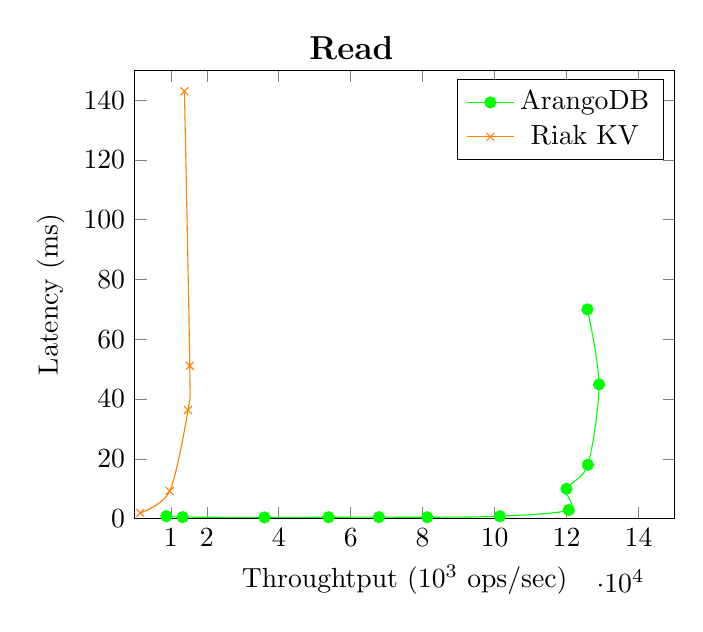
\begin{tikzpicture}
\begin{axis}[
    xlabel=Throughtput ($10^{3}$ ops/sec),
    ylabel=Latency (ms),
    xmin=0, xmax=15000,
    ymin=0, ymax=150,
    xtick={1000, 2000,4000, 6000, 8000,10000,12000, 14000},
    xticklabels={1, 2, 4, 6, 8, 10, 12, 14},
    ytick={0,20,...,160}
            ]
\addplot[smooth,color=green,mark=*] plot coordinates {
    (876,0.8)
    (1329,0.5)
    (3603,0.4)
    (5385,0.45)
    (6782,0.49)
    (8127,0.45)
    (10145,0.8)
    (12062, 2.9)
    (11995, 9.961)
    (12592, 18)
    (12903, 44.884)
    (12581, 70)
};
\addlegendentry{ArangoDB}

\addplot[smooth,color=orange,mark=x]
    plot coordinates {
    (149,1.9)
    (969,9.219)
    (1476,36.330)
    (1526,51.128)
    (1378,142.990)
    };
\addlegendentry{Riak KV}
\end{axis}
\node[above,font=\large\bfseries] at (current bounding box.north) {Read};

    \end{tikzpicture}


% Second diagram Workload a - write operations
    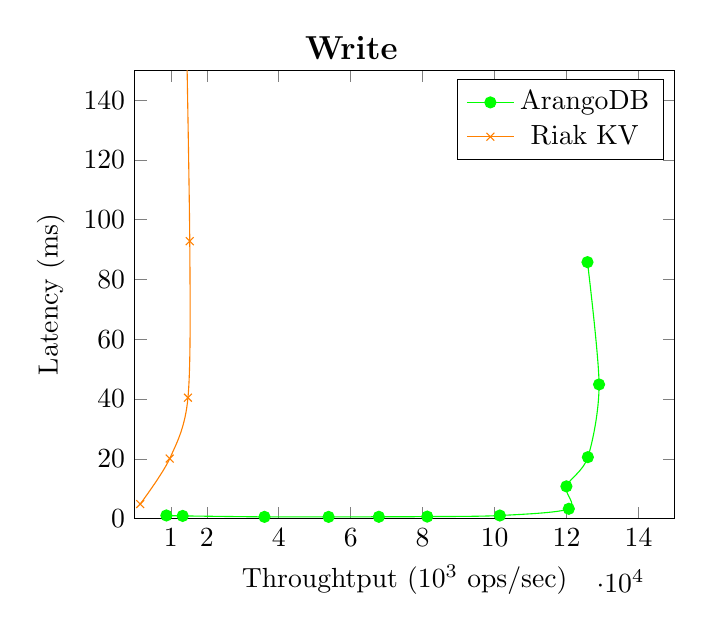
\begin{tikzpicture}
\begin{axis}[
    xlabel=Throughtput ($10^{3}$ ops/sec),
    ylabel=Latency (ms),
    xmin=0, xmax=15000,
    ymin=0, ymax=150,
    xtick={1000, 2000,4000, 6000, 8000,10000,12000, 14000},
    xticklabels={1, 2, 4, 6, 8, 10, 12, 14},
    ytick={0,20,...,160}
            ]
\addplot[smooth,color=green,mark=*] plot coordinates {
    (876,1.046)
    (1329,0.902)
    (3603,0.582)
    (5385, 0.577)
    (6782, 0.609)
    (8127, 0.670)
    (10145, 1.031)
    (12062, 3.279)
    (11995,  10.787)
    (12592, 20.565)
    (12903, 44.884)
    (12581, 85.810)
};
\addlegendentry{ArangoDB}

\addplot[smooth,color=orange,mark=x]
    plot coordinates {
        (149, 4.867)
        (969, 20.091)
        (1476, 40.452)
        (1526,92.816)
        (1378,198.836)
    };
\addlegendentry{Riak KV}
\end{axis}

\node[above,font=\large\bfseries] at (current bounding box.north) {Write};
    \end{tikzpicture}

    
\subsection{Workload b}
    To Workload B είναι heavy Read (95/100 Read - 5/100 Updates) και μία εφαρμογή του είναι η προσθήκη ετικετών σε φωτογραφίες (photo tagging) όπου η προσθήκη tag είναι ένα Update όμως κυρίως είναι η ανάγνωση ετικετών. Πάλι η ArangoDB είχε μεγαλύτερο throughput και μικρότερο latency. To μέγιστο throughput της ArangoDB ήταν λίγο καλύτερο στην περίπτωση του Workload A από το Workload B.

%Third Diagram Workload b
%  Read s
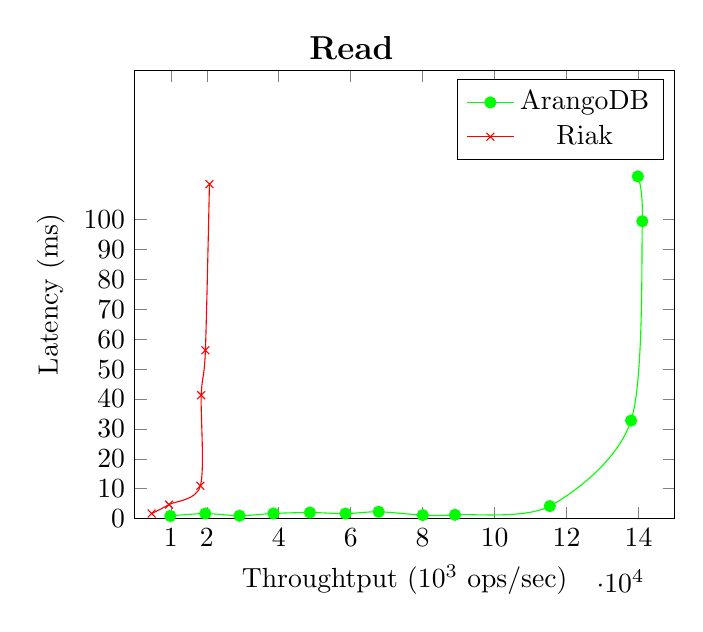
\begin{tikzpicture}
    \begin{axis}[
        xlabel=Throughtput ($10^{3}$ ops/sec),
        ylabel=Latency (ms),
        xmin=0, xmax=15000,
        ymin=0, ymax=150,
        xtick={1000, 2000,4000, 6000, 8000,10000,12000, 14000},
        xticklabels={1, 2, 4, 6, 8, 10, 12, 14},
        ytick={0,10,...,100}
                ]
    \addplot[smooth,mark=*,green] plot coordinates {
        (987,0.9)
        (1957,1.69)
        (2909,0.96)
        (3850,1.72)
        (4866,2.04)
        (5854,1.67)
        (6777,2.29)
        (8003, 1.17)
        (8898, 1.27)
        (11534, 4.19)
        (13793, 32.810)
        (14105, 99.5)
        (13981,114.5)
    };
    \addlegendentry{ArangoDB}
    
    \addplot[smooth,color=red,mark=x]
        plot coordinates {
            (466.8,1.69)
            (950.9,4.7)
            (1821,10.98)
            (1844,41.29)
           (1961,56.31)
           (2073,111.9)
            
        };
    \addlegendentry{Riak}
    \end{axis}
    \node[above,font=\large\bfseries] at (current bounding box.north) {Read};
    
        \end{tikzpicture}

%Fourth Diagram Workload b Update
%  Read s
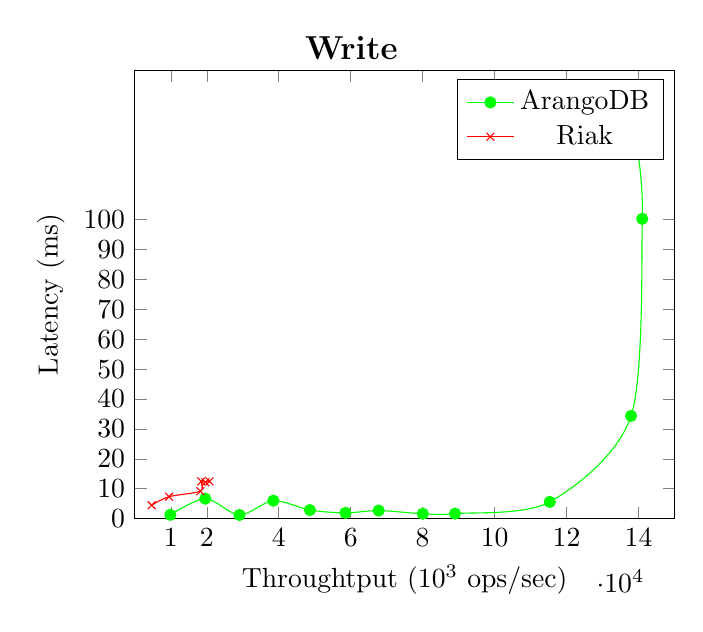
\begin{tikzpicture}
    \begin{axis}[
        xlabel=Throughtput ($10^{3}$ ops/sec),
        ylabel=Latency (ms),
        xmin=0, xmax=15000,
        ymin=0, ymax=150,
        xtick={1000, 2000,4000, 6000, 8000,10000,12000, 14000},
        xticklabels={1, 2, 4, 6, 8, 10, 12, 14},
        ytick={0,10,...,100}
                ]
    \addplot[smooth,mark=*,green] plot coordinates {
        (987,1.26)
        (1957,6.66)
        (2909,1.214)
        (3850,5.99)
        (4866,2.86)
        (5854,1.92)
        (6777,2.69)
        (8003, 1.64)
        (8898, 1.669)
        (11534, 5.596)
        (13793, 34.36)
        (14105, 100.3)
        (13981,122.1)
    };
    \addlegendentry{ArangoDB}
    
    \addplot[smooth,color=red,mark=x]
        plot coordinates {
            (466.8,4.49)
            (950.9,7.33)
            (1821,9.17)
            (1844,12.46)
           (1961,12.17)
           (2073,12.45)
            
        };
    \addlegendentry{Riak}
    \end{axis}
    \node[above,font=\large\bfseries] at (current bounding box.north) {Write};
    
        \end{tikzpicture}

\subsection{Διπλασιάζοντας του πόρους της Riak}

\subsubsection{Workload a - Updates}
Από το worklfow a θα συγκρίνουμε τις επιδόσεις στα reads, μιας και τα reads θα εξετασθούν από το heavy-read workflow b.

%Fifth Diagram Workload a Update
%  Writes
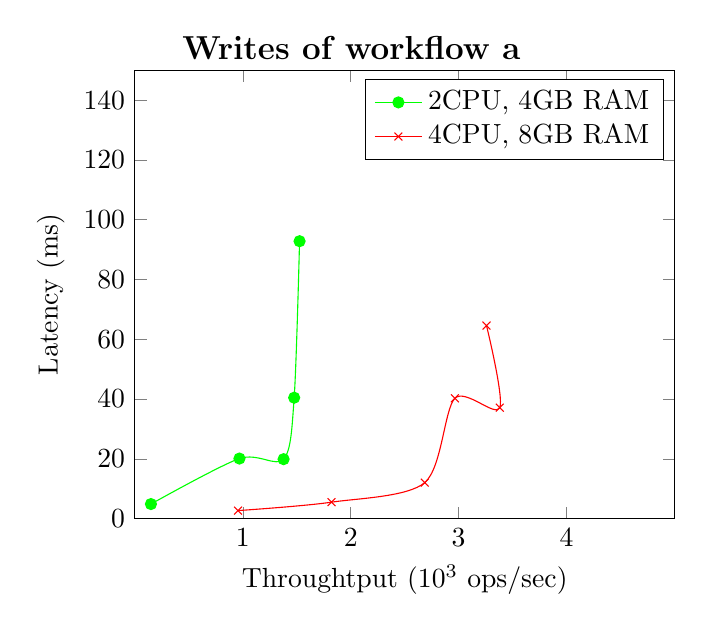
\begin{tikzpicture}
    \begin{axis}[
        xlabel=Throughtput ($10^{3}$ ops/sec),
        ylabel=Latency (ms),
        xmin=0, xmax=5000,
        ymin=0, ymax=150,
        xtick={1000,2000,3000, 4000},
        xticklabels={1,2,3, 4},   % <---
        ytick={0,20,...,150}
                ]
    \addplot[smooth,mark=*,green] plot coordinates {
        (149, 4.867)
        (969, 20.091)
        (1378,19.8836)
        (1476, 40.452)
        (1526,92.816)

    };
    \addlegendentry{2CPU, 4GB RAM}
    
    \addplot[smooth,color=red,mark=x]
        plot coordinates {
            (956, 2.686)
            (1822, 5.497)
            (2686, 12.037)
            (2965, 40.240)
            (3381, 37.114)
            (3258, 64.592)
        };
    \addlegendentry{4CPU, 8GB RAM}
    \end{axis}
    \node[above,font=\large\bfseries] at (current bounding box.north) {Writes of workflow a};
    
        \end{tikzpicture}


\subsubsection{Workload b - Reads}
%Sixth Diagram Workload b Reads
%  Read s
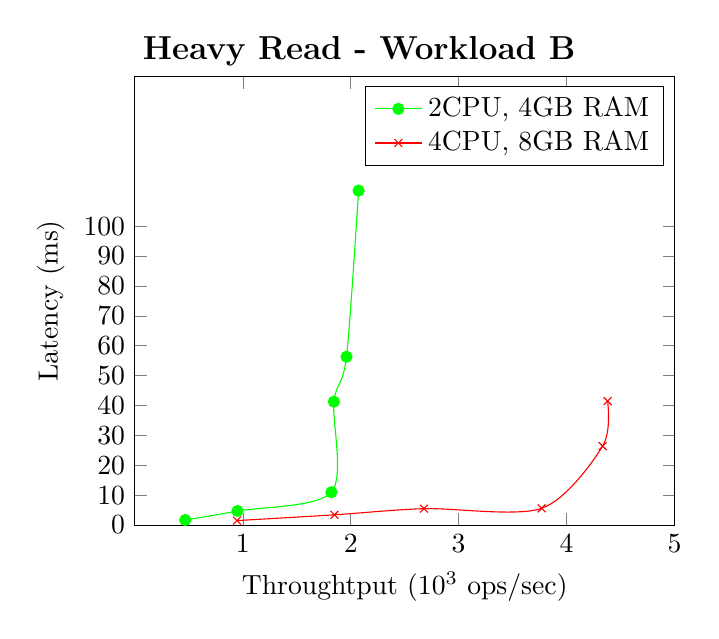
\begin{tikzpicture}
    \begin{axis}[
        xlabel=Throughtput ($10^{3}$ ops/sec),
        ylabel=Latency (ms),
        xmin=0, xmax=5000,
        ymin=0, ymax=150,
        xtick={1000, 2000, 3000, 4000, 5000},
        xticklabels={1,2, 3, 4, 5 },   % <---
        ytick={0,10,...,100}
                ]
    \addplot[smooth,mark=*,green] plot coordinates {
        (466.8,1.69)
        (950.9,4.7)
        (1821,10.98)
        (1844,41.29)
        (1961,56.31)
        (2073,111.9)


    };
    \addlegendentry{2CPU, 4GB RAM}
    
    \addplot[smooth,color=red,mark=x]
        plot coordinates {
            (946.7,1.5)
            (1849,3.43)
            (2679,5.49)
            (3769,5.6)
            (4334,26.4)
            (4380,41.48)
            
        };
    \addlegendentry{4CPU, 8GB RAM}
    \end{axis}
    \node[above,font=\large\bfseries] at (current bounding box.north) {Heavy Read - Workload B};
    
        \end{tikzpicture}


Όπως συμβαίνει με κάθε συγκριτική αξιολόγηση, η δυνατότητα εφαρμογής των 
αποτελεσμάτων σε μια εφαρμογή δεν είναι πάντα σαφής. Οι περιπτώσεις χρήσης για 
ArangoDB και Riak-KV είναι ποικίλες και είναι σημαντικό να χρησιμοποιηθούν
δοκιμές απόδοσης που αντικατοπτρίζουν τις ανάγκες της εφαρμογής και του υλικού που θα 
χρησιμοποιηθεί για την ανάπτυξή της.  
Μόνο οι εφαρμογές σας, τα δεδομένα σας και η υποδομή σας μπορούν να σας πουν 
τι πρέπει να γνωρίζετε και ποια τεχνολογία να επιλέξετε. 

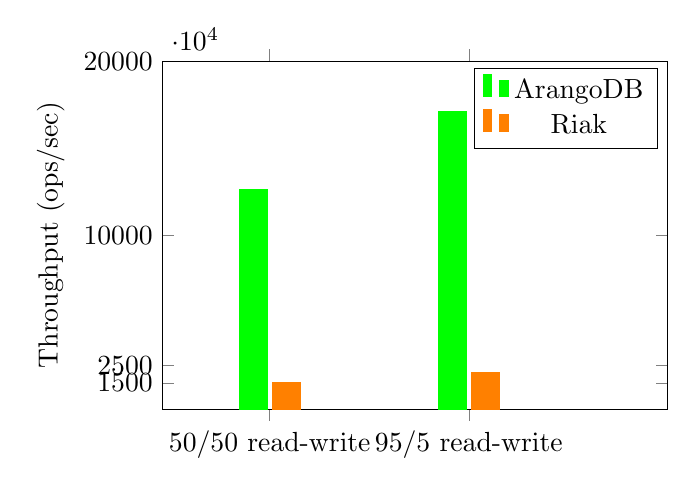
\begin{tikzpicture}
 
    \begin{axis} [ybar,height=6cm,width=8cm,
        ylabel=Throughput (ops/sec),
        xmin={0}, xmax={3.3},
        xtick={0.7, 2},
        xticklabels={50/50 read-write, 95/5 read-write},
        ymin=0, ymax=20000,
        ytick={1500,2500, 10000, 20000},
        yticklabels={1500,2500, 10000, 20000 }   % <---
        ]
    \addplot[color=green, fill=green ] coordinates{
        (0.7,12592) 
        (2,17105) 
    };

    \addlegendentry{ArangoDB}
    \addplot[color=orange, fill=orange]  coordinates {(0.7,1526) (2,2073)};
    \addlegendentry{Riak}

    \end{axis}
\end{tikzpicture}


Το συμπέρασμα από τα test που πραγματοποίηθηκαν είναι οτι η ArangoDB είναι
αρκετά γρήγορη για να χρησιμοποιηθεί σε μια εφαρμογή που χρειάζεται να αποθηκεύει
και να διαχειρίζεται μεγάλα δεδομένα. Επίσης, η ArangoDB είναι πολύ εύκολη στην
χρήση και στην εγκατάσταση. Επιπλέον, η ArangoDB διαθέτει επιπλέον λειτουργίες
που δεν υπάρχουν στο Riak-KV.
Αυτές οι λειτουργίες είναι η δυνατότητα
αναζήτησης στα δεδομένα, η δυνατότητα δημιουργίας ερωτημάτων σε μορφή
γραμμής εντολών,η μοντελοποίηση των δεδομένων σε γράφους. 
Σε συνάρτηση με τους διαθέσιμους πόρους, η ArangoDB μπορεί να
είναι πιο αποδοτική από τη  Riak-KV. 

Αντίθετα, η Riak-KV είναι ανεκτική σε 
network partitions και σε σφάλματα κόμβων όπου είναι σχεδόν εγγυημένη η πρόσβαση
στα δεδομένα μας. Ο κάθε χρήστης θα πρέπει να κάνει τη δική του επιλογή 
σύμφωνα με τις μη λειτουργικές απαιτήσεις της εφαρμογής του. Αν προτεραιότητα είναι ο μικρός 
χρόνος απόκρισης και η εξυπηρέτηση πολλών αιτημάτων ταυτόχρονα, σε σύστημα περιορισμένων πόρων
τότε η ArangoDB μοιάζει καλή επιλογή. Χωρίς αυτό να σημαίνει πως η Riak KV δεν μπορεί να χρησιμοποιηθεί
κάτω από συνθήκες μεγάλης φόρτωσης. Η σχεδόν γραμμική αύξηση της απόδοσης της Riak KV με τον αριθμό των
με τη προσθήκη κόμβων, μπορεί να μας δώσει την εντύπωση ότι η Riak KV μπορεί να χρησιμοποιηθεί και σε
συστήματα με μεγάλη φόρτωση. 
Επίσης και στην arango μπορουύμε να πετύχουμε γραμμικά οριζόντια κλιμάκωση αν το 
sharding γίνεται αποκλειστικά σε επίπεδο κλειδιών των δεδομένων. Αντίθετα αν το sharding γίνεται χρησιμοποιώντας 
διαφορετικά shard κλειδιά, τότε χρειάζεται να γίνει αναζήτηση σε όλα τα shard και η απόδοση 
μπορεί να μην κλιμακώνεται γραμμικά.
\section{βιβλιογραφία και παραπομπές που χρησιμοποιήθηκαν στο κείμενο}

\section*{References}

Please number citations consecutively within brackets \cite{b1}. The 
sentence punctuation follows the bracket \cite{b2}. Refer simply to the reference 
number, as in \cite{b3}---do not use ``Ref. \cite{b3}'' or ``reference \cite{b3}'' except at 
the beginning of a sentence: ``Reference \cite{b3} was the first $\ldots$''

Number footnotes separately in superscripts. Place the actual footnote at 
the bottom of the column in which it was cited. Do not put footnotes in the 
abstract or reference list. Use letters for table footnotes.

Unless there are six authors or more give all authors' names; do not use 
``et al.''. Papers that have not been published, even if they have been 
submitted for publication, should be cited as ``unpublished'' \cite{b4}. Papers 
that have been accepted for publication should be cited as ``in press'' \cite{b5}. 
Capitalize only the first word in a paper title, except for proper nouns and 
element symbols.

For papers published in translation journals, please give the English 
citation first, followed by the original foreign-language citation \cite{b6}.

\begin{thebibliography}{00}
\bibitem{b1} G. Eason, B. Noble, and I. N. Sneddon, ``On certain integrals of Lipschitz-Hankel type involving products of Bessel functions,'' Phil. Trans. Roy. Soc. London, vol. A247, pp. 529--551, April 1955.
\bibitem{b2} J. Clerk Maxwell, A Treatise on Electricity and Magnetism, 3rd ed., vol. 2. Oxford: Clarendon, 1892, pp.68--73.
\bibitem{b3} I. S. Jacobs and C. P. Bean, ``Fine particles, thin films and exchange anisotropy,'' in Magnetism, vol. III, G. T. Rado and H. Suhl, Eds. New York: Academic, 1963, pp. 271--350.
\bibitem{b4} K. Elissa, ``Title of paper if known,'' unpublished.
\bibitem{b5} R. Nicole, ``Title of paper with only first word capitalized,'' J. Name Stand. Abbrev., in press.
\bibitem{b6} Y. Yorozu, M. Hirano, K. Oka, and Y. Tagawa, ``Electron spectroscopy studies on magneto-optical media and plastic substrate interface,'' IEEE Transl. J. Magn. Japan, vol. 2, pp. 740--741, August 1987 [Digests 9th Annual Conf. Magnetics Japan, p. 301, 1982].
\bibitem{b7} M. Young, The Technical Writer's Handbook. Mill Valley, CA: University Science, 1989.
\end{thebibliography}
\vspace{12pt}
\color{red}
IEEE conference templates contain guidance text for composing and formatting conference papers. Please ensure that all template text is removed from your conference paper prior to submission to the conference. Failure to remove the template text from your paper may result in your paper not being published.

\end{document}
